\ifdefined\included
\else
\documentclass[english,a4paper,11pt,twoside]{StyleThese}
\usepackage{amsmath,amssymb}             % AMS Math
\usepackage[T1]{fontenc}
\usepackage[utf8x]{inputenc}
\usepackage{babel}
\usepackage{datetime}

\usepackage{lmodern}
\usepackage{tabularx}
%\usepackage{tabular}
\usepackage{multirow}

\usepackage{subfigure}
\usepackage{fancyvrb}
\usepackage{algorithmic}
\usepackage{algorithm}
\usepackage{mathtools}


\usepackage{hhline}
\usepackage[left=1.5in,right=1.3in,top=1.1in,bottom=1.1in,includefoot,includehead,headheight=13.6pt]{geometry}
\renewcommand{\baselinestretch}{1.05}

% Table of contents for each chapter

\usepackage[nottoc, notlof, notlot]{tocbibind}
\usepackage{minitoc}
\setcounter{minitocdepth}{2}
\mtcindent=15pt
% Use \minitoc where to put a table of contents

\usepackage{aecompl}


% Glossary / list of abbreviations

\usepackage[intoc]{nomencl}
\iftoggle{ThesisInEnglish}{%
\renewcommand{\nomname}{Glossary}
}{ %
\renewcommand{\nomname}{Liste des Abréviations}
}

\newcommand{\accom}[1]{\textcolor{red}{[#1]}}

\makenomenclature

% My pdf code

\usepackage{ifpdf}

\ifpdf
  \usepackage[pdftex]{graphicx}
  \DeclareGraphicsExtensions{.jpg}
  \usepackage[a4paper,pagebackref,hyperindex=true]{hyperref}
  \usepackage{tikz}
  \usetikzlibrary{arrows,shapes,calc}
\else
  \usepackage{graphicx}
  \DeclareGraphicsExtensions{.ps,.eps}
  \usepackage[a4paper,dvipdfm,pagebackref,hyperindex=true]{hyperref}
\fi

\graphicspath{{.}{images/}}

%% nicer backref links. NOTE: The flag ThesisInEnglish is used to define the
% language in the back references. Read more about it in These.tex

\iftoggle{ThesisInEnglish}{%
\renewcommand*{\backref}[1]{}
\renewcommand*{\backrefalt}[4]{%
\ifcase #1 %
(Not cited.)%
\or
(Cited in page~#2.)%
\else
(Cited in pages~#2.)%
\fi}
\renewcommand*{\backrefsep}{, }
\renewcommand*{\backreftwosep}{ and~}
\renewcommand*{\backreflastsep}{ and~}
}{%
\renewcommand*{\backref}[1]{}
\renewcommand*{\backrefalt}[4]{%
\ifcase #1 %
(Non cité.)%
\or
(Cité en page~#2.)%
\else
(Cité en pages~#2.)%
\fi}
\renewcommand*{\backrefsep}{, }
\renewcommand*{\backreftwosep}{ et~}
\renewcommand*{\backreflastsep}{ et~}
}

% Links in pdf
\usepackage{color}
\definecolor{linkcol}{rgb}{0,0,0.4} 
\definecolor{citecol}{rgb}{0.5,0,0} 
\definecolor{linkcol}{rgb}{0,0,0} 
\definecolor{citecol}{rgb}{0,0,0}
% Change this to change the informations included in the pdf file

\hypersetup
{
bookmarksopen=true,
pdftitle="Joint Action for Human-Robot Interaction",
pdfauthor="Sandra DEVIN", %auteur du document
pdfsubject="Thesis", %sujet du document
%pdftoolbar=false, %barre d'outils non visible
pdfmenubar=true, %barre de menu visible
pdfhighlight=/O, %effet d'un clic sur un lien hypertexte
colorlinks=true, %couleurs sur les liens hypertextes
pdfpagemode=None, %aucun mode de page
pdfpagelayout=SinglePage, %ouverture en simple page
pdffitwindow=true, %pages ouvertes entierement dans toute la fenetre
linkcolor=linkcol, %couleur des liens hypertextes internes
citecolor=citecol, %couleur des liens pour les citations
urlcolor=linkcol %couleur des liens pour les url
}

% definitions.
% -------------------

\setcounter{secnumdepth}{3}
\setcounter{tocdepth}{2}

% Some useful commands and shortcut for maths:  partial derivative and stuff

\newcommand{\pd}[2]{\frac{\partial #1}{\partial #2}}
\def\abs{\operatorname{abs}}
\def\argmax{\operatornamewithlimits{arg\,max}}
\def\argmin{\operatornamewithlimits{arg\,min}}
\def\diag{\operatorname{Diag}}
\newcommand{\eqRef}[1]{(\ref{#1})}

\usepackage{rotating}                    % Sideways of figures & tables
%\usepackage{bibunits}
%\usepackage[sectionbib]{chapterbib}          % Cross-reference package (Natural BiB)
%\usepackage{natbib}                  % Put References at the end of each chapter
                                         % Do not put 'sectionbib' option here.
                                         % Sectionbib option in 'natbib' will do.
\usepackage{fancyhdr}                    % Fancy Header and Footer

% \usepackage{txfonts}                     % Public Times New Roman text & math font
  
%%% Fancy Header %%%%%%%%%%%%%%%%%%%%%%%%%%%%%%%%%%%%%%%%%%%%%%%%%%%%%%%%%%%%%%%%%%
% Fancy Header Style Options

\pagestyle{fancy}                       % Sets fancy header and footer
\fancyfoot{}                            % Delete current footer settings

%\renewcommand{\chaptermark}[1]{         % Lower Case Chapter marker style
%  \markboth{\chaptername\ \thechapter.\ #1}}{}} %

%\renewcommand{\sectionmark}[1]{         % Lower case Section marker style
%  \markright{\thesection.\ #1}}         %

\fancyhead[LE,RO]{\bfseries\thepage}    % Page number (boldface) in left on even
% pages and right on odd pages
\fancyhead[RE]{\bfseries\nouppercase{\leftmark}}      % Chapter in the right on even pages
\fancyhead[LO]{\bfseries\nouppercase{\rightmark}}     % Section in the left on odd pages

\let\headruleORIG\headrule
\renewcommand{\headrule}{\color{black} \headruleORIG}
\renewcommand{\headrulewidth}{1.0pt}
\usepackage{colortbl}
\arrayrulecolor{black}

\fancypagestyle{plain}{
  \fancyhead{}
  \fancyfoot{}
  \renewcommand{\headrulewidth}{0pt}
}

%\usepackage{MyAlgorithm}
%\usepackage[noend]{MyAlgorithmic}
\usepackage[ED=MITT - STICIA, Ets=INP]{tlsflyleaf}
%%% Clear Header %%%%%%%%%%%%%%%%%%%%%%%%%%%%%%%%%%%%%%%%%%%%%%%%%%%%%%%%%%%%%%%%%%
% Clear Header Style on the Last Empty Odd pages
\makeatletter

\def\cleardoublepage{\clearpage\if@twoside \ifodd\c@page\else%
  \hbox{}%
  \thispagestyle{empty}%              % Empty header styles
  \newpage%
  \if@twocolumn\hbox{}\newpage\fi\fi\fi}

\makeatother
 
%%%%%%%%%%%%%%%%%%%%%%%%%%%%%%%%%%%%%%%%%%%%%%%%%%%%%%%%%%%%%%%%%%%%%%%%%%%%%%% 
% Prints your review date and 'Draft Version' (From Josullvn, CS, CMU)
\newcommand{\reviewtimetoday}[2]{\special{!userdict begin
    /bop-hook{gsave 20 710 translate 45 rotate 0.8 setgray
      /Times-Roman findfont 12 scalefont setfont 0 0   moveto (#1) show
      0 -12 moveto (#2) show grestore}def end}}
% You can turn on or off this option.
% \reviewtimetoday{\today}{Draft Version}
%%%%%%%%%%%%%%%%%%%%%%%%%%%%%%%%%%%%%%%%%%%%%%%%%%%%%%%%%%%%%%%%%%%%%%%%%%%%%%% 

\newenvironment{maxime}[1]
{
\vspace*{0cm}
\hfill
\begin{minipage}{0.5\textwidth}%
%\rule[0.5ex]{\textwidth}{0.1mm}\\%
\hrulefill $\:$ {\bf #1}\\
%\vspace*{-0.25cm}
\it 
}%
{%

\hrulefill
\vspace*{0.5cm}%
\end{minipage}
}

\let\minitocORIG\minitoc
\renewcommand{\minitoc}{\minitocORIG \vspace{1.5em}}

\usepackage{multirow}
%\usepackage{slashbox}

\newenvironment{bulletList}%
{ \begin{list}%
	{$\bullet$}%
	{\setlength{\labelwidth}{25pt}%
	 \setlength{\leftmargin}{30pt}%
	 \setlength{\itemsep}{\parsep}}}%
{ \end{list} }

\newtheorem{definition}{Définition}
\renewcommand{\epsilon}{\varepsilon}

% centered page environment

\newenvironment{vcenterpage}
{\newpage\vspace*{\fill}\thispagestyle{empty}\renewcommand{\headrulewidth}{0pt}}
{\vspace*{\fill}}

\usepackage{tablefootnote}

\sloppy
\begin{document}
\setcounter{chapter}{4} %% Numéro du chapitre précédent ;)
\dominitoc
\faketableofcontents
\fi

\chapter{Evaluation of the global system}
\minitoc

\label{ch:Eval}

\section{Motivations}

In the two previous chapters, we presented several ameliorations on the way the robot elaborates and executes Shared Plans. We first endowed the robot with the ability to take into account humans mental states during Shared Plans execution. In a second time, we saw how the robot is able to compute more flexible Shared Plans where it identifies which decisions have to be taken at planning time and which one are better to be postponed. Then, the robot is able to take these decisions while smoothly adapting to the human choices. 

These two ameliorations have been quantitatively and independently evaluated in simulation. In this chapter, we want to evaluate the global system including both ameliorations. Moreover, in addition to quantitative results, we want to evaluate the acceptance of the system by real users. To do so, we defined a task which allows to highlight the benefits of the system. This task has been used to evaluate the global system in simulation in order to get quantitative results. Then, the same task (with minor modifications) has been used during a user study in the real robot in order to get a subjective evaluation of the global system. 

\section{Task}

\label{sec:task_us}

The task used for the global evaluation is inspired from the "Inventory scenario" of Chapter~\ref{ch:MS}. In the task, the human and the robot have to scan several colored cubes and store them into a box of the same color. At the beginning of the interaction, both agents have a stack of colored cubes they can access (and only them can access). There are blue, green and red cubes. The stack of the human is located in another room, in a way that, to get an object, the human has to leave the sight of view of the robot (see Fig.~\ref{fig:setUpSimu}). For the cubes to be scanned, the agents need to put them on one of the two possible areas on the table in front of the robot (see Fig.~\ref{fig:setUpSimu}). Once a cube is on an area, the robot can scan it by orienting its head and turning on a red light in the direction of the object (see Fig.é\ref{fig:scan}). If the robot scans an object while the human is not looking at him (e.g. he is in another room to pick a cube), the human will not be aware that the object has been scanned unless the robot tells him. Once the cube scanned, it can be stored in a box of the same color (e.g. the blue cubes in a blue box). The robot has access to a blue box, the human to a green box, and both have access to a red box. Consequently, only the robot can store the blue cubes, only the human can store the green cubes and both can store the red cubes. As well as for his stack, the boxes of the human are located in another room (see Fig.~\ref{fig:setUpSimu}). 


\begin{figure}[!h]
	\centering
    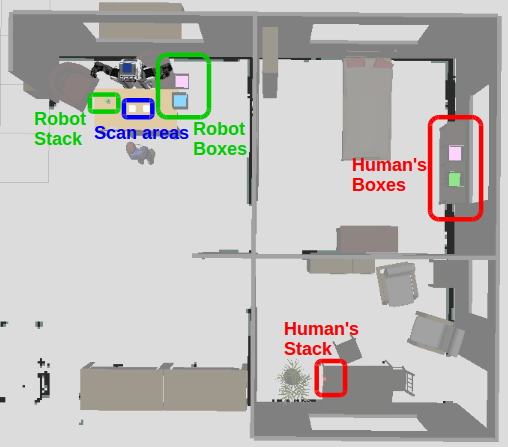
\includegraphics[width=0.9\textwidth]{figs/Chapter5/SetUpSimu.png}
    \caption{Set-up for the task used during evaluation. The human and the robot need to take the cubes from their stack and put them in the scan areas. Once a cube is in a scan area, the robot can scan it. Then, the agents can store the cubes in the boxes of the same color. The human has access to a green and a red box and the robot has access to a blue and a red box.}
    \label{fig:setUpSimu}
\end{figure}

Both in simulation and in the user study, we compared 4 different conditions:
\begin{itemize}
\item using the original system, called Reference System (RS), with all decisions and instantiations performed at planning time and no estimation of the human mental state:
\begin{itemize}
\item \textbf{RS-none mode:} the robot verbalizes nothing (unless it is strictly necessary)
\item \textbf{RS-all mode:} the robot informs the human when he has to perform an action, when it will act and about all actions he missed.
\end{itemize}
\item using the proposed system, called New System (NS): 
\begin{itemize}
\item \textbf{NS-N:} the robot uses the \textbf{Negotiation} mode previously defined when a decision needs to be made concerning \textit{X agent} action,
\item \textbf{NS-A:} the robot uses the \textbf{Adaptation} mode.
\end{itemize}
\end{itemize}

\section{Evaluation in simulation}

\subsection{Modalities}

We first evaluated our system in simulation. Different set-ups were used as initial state of the task: we randomized the composition of the stack of the human and the robot. In each case there was three cubes of each color (red, blue and green) and the robot stack was composed of 4 cubes and the human one of 5 cubes. The dispositions of the cubes in the stacks were randomized. The robot was confronted to a simulated human with different kinds of behaviors. In all cases, the human was acting as bellow:
\begin{itemize}
\item when the human is in front of the robot with no cube in hand and there is a green cube he knows it is scanned, it goes to the boxes to store it.
\item whenever the human is idle with no cube in hand, it goes to his stack to pick a cube and then comes back to the table.
\item if the human has a cube in hand to be scanned, he put it on a scan area (if free). If there is no free area, the human waits in front of the robot.
\item if the human has no more cube in his stack he waits in front of the robot.
\end{itemize}
When the human is in front of the robot with no cube in hand and there is a red cube he knows it is scanned, the human chooses:
\begin{itemize}
\item to store it systematically (\textbf{hurry-case})
\item not to store it systematically (\textbf{lazy-case})
\item to store it with 50\% chance (\textbf{50\%-case})
\end{itemize}
Then, we settled two different human behaviors:
\begin{itemize}
\item \textbf{the "kind" human (case=K)} who adapts his behavior to what the robot verbalizes (i.e. does an action if the robot asks him and does not execute the actions the robot says it will perform)
\item \textbf{the "stubborn" human (case=S)} who does not react nor comply to robot verbalization (he will not change his decision whatever the robot says).
\end{itemize}
In all cases, the human answers to the robot questions concerning the red cubes with the answer corresponding to his decision.


We measured:
\begin{itemize}
\item \textit{the number of verbal interactions} between the human and the robot (either an information given by the robot or question asked), in Tab.~\ref{tab:incompatibleDecisions}.
\item \textit{the number of human/robot incompatible decisions}: either both decide to perform the same action (and the robot stops its own action to avoid the conflict) or both decide not to perform the action (the robot first asks the human to perform the action after a predefined time and, if after another period the human has still not executed the action, the robot looks for a new plan where it can proceed), in Tab.~\ref{tab:verbalInteraction}.
\item \textit{the total execution time:} for the human and the robot to perform the task, in Fig.~\ref{fig:resTime}.
\end{itemize}

\subsection{Results}

\begin{table*}[!h]
\centering
  \begin{tabular}{|c||c|c|c|c|}
  \hline
     & \textbf{RS-none} & \textbf{RS-all} & \textbf{Neg} & \textbf{Adapt} \\
  \hline
  \hline
     \textbf{50\%-K} & 2.4 (0.84) & 20.7 (1.34) & 3.4 (1.51) & 2 (1.33) \\
  \hline
     \textbf{hurry-K} & 1.8 (0.79) & 21.1 (2.08) & 1.9 (1.10) & 2.2 (1.13) \\
  \hline
     \textbf{lazy-K} & 3.0 (1.33) & 21 (1.56) & 3.3 (1.42) & 1.6 (1.17) \\
  \hline
     \textbf{50\%-S} & 2.5 (1.43) & 23.9 (1.59) & 3.3 (1.49) & 1.7 (0.95)\\
  \hline
     \textbf{hurry-S} & 1.5 (0.97) & 20.9 (1.29) & 2.4 (1.89) & 1.9 (0.99)\\
  \hline
     \textbf{lazy-S} & 3.2 (0.92) & 25.2 (1.55) & 2.8 (1.68) & 1.8 (1.14)\\
  \hline
  \end{tabular}
   \caption{Results for the reference system (RS) and the proposed system (NS-N for the negotiation mode and NS-A for the adaptation mode). Number of verbal interactions (i.e. question asked by the robot in the negotiation mode or an information given with the reference system). The numbers correspond to means in 10 runs and their associated standard deviations.}
   \label{tab:verbalInteraction}
\end{table*}

\paragraph{RS-none performance:} Even if the robot is supposed not to speak in this mode, we can see in Tab.~\ref{tab:verbalInteraction} that there are still verbalizations, especially in the cases where the human is lazy. These verbal interactions are due to two reasons. First, when the robot decides that the human should store a red cube and the human decides he will not do it, the robot unlocks the situation by asking the human to store the object (and in the stubborn case, as the human will still not do it, it then changes its plan). Secondly, when the human does not see that a cube has been scanned he will wait before storing it. As previously, the robot unlocks the situation by asking the human to store the object (as it detects that the human is not executing his action). 

This mode is also the mode where there are the most incompatible decisions as the robot verbalize nothing. These incompatible decisions are mainly conflicts concerning the red cubes to store and the scan areas (as there is no notions of \textit{similar} objects in this mode, the robot stops its actions if the human puts a cube in the same area it was aiming for even if the other is free).

Concerning the execution time, this mode is the one with the highest ones. The execution times are especially high in the stubborn and lazy cases, as, when the human decides not to store a cube, the robot wastes time to ask the human to do it and only then looks for a new plan where it stores the cube. 

\begin{table*}[!h]
\centering
  \begin{tabular}{|c||c|c|c|c|}
  \hline
     & \textbf{RS-none} & \textbf{RS-all} & \textbf{NS-N} & \textbf{NS-A} \\
  \hline
  \hline
     \textbf{50\%-K} & 2.9 (0.99) & 0.9 (0.57) & 0.6 (0.7) & 0.3 (0.48) \\
  \hline
     \textbf{hurry-K} & 2.5 (0.97) & 1.0 (0.94) & 0.6 (0.52) & 0.4 (0.52)\\
  \hline
     \textbf{lazy-K} & 3.5 (1.08) & 0.8 (0.63) & 0.5 (0.7) & 0.5 (0.53) \\
  \hline
     \textbf{50\%-S} & 2.9 (1.45) & 1.9 (0.99) & 0.6 (0.52) & 0.5 (0.97) \\
  \hline
     \textbf{hurry-S} & 2.3 (1.34) & 1.0 (0.82) & 0.5 (0.53) & 0.4 (0.52) \\
  \hline
     \textbf{lazy-S} & 3.5 (0.97) & 2.6 (1.84) & 0.3 (0.67) & 0.4 (0.52)  \\
  \hline
  \end{tabular}
   \caption{Results for the reference system (RS) and the proposed system (NS-N for the negotiation mode and NS-A for the adaptation mode). Number of incompatible decisions between the human and the robot (i.e. either both agents decide to perform the same action or both decide not to perform a given action). The numbers correspond to means in 10 runs and their associated standard deviations.}
   \label{tab:incompatibleDecisions} 
\end{table*}

\paragraph{RS-all performance:}
In this mode, as expected, there is a lot of verbal interactions. Indeed, the robot informs not only about who should perform the actions but also about all actions that the human missed. However, even with the "kind" human, it is not enough to get ride of all conflicts. Indeed, there are still conflicts concerning the scan areas as the robot has to stop its action if the human puts his cube in the area it was aiming for. There are even more conflicts with the "stubborn" human as, even if the robot gives information, the human does not change his choices.

Concerning the execution times, they are low for the "kind" human as the human follows what the robot asks. However, with the "stubborn" human (not with the "hurry" one as the human takes the initiative to execute all possible actions), the execution times become higher. Indeed, when the robot has decided that the human has to perform an action, the robot wastes time to wait for the human to perform it before looking for another plan. These execution times are still lower than with RS-NONE because, as the robot informs for all missed actions, there is no time where the human waits to know that a cube has been scanned.

\begin{figure}[!h]
	\centering
    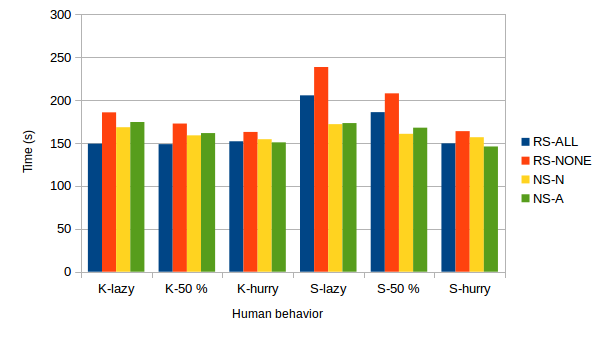
\includegraphics[width=0.9\textwidth]{figs/Chapter5/Time.png}
    \caption{Time in seconds each system spent performing the task for each kind of human behavior (mean in 10 runs).}
    \label{fig:resTime}
\end{figure}


\paragraph{New system performance:}
We can see that the performance of the new system is globally better than in the two other modes. Concerning the incompatible decisions, it only remains the conflicts when the human puts a cube on the last available scan area and the robot was trying to put an object on it too. The execution times are lower than the reference system when the human is stubborn. Indeed, the robot does not wait for the human to perform actions he does not want to execute (it either asks or adapts). Moreover, as the robot informs the human about the cube which has been scanned during his absence (and which the human can store), the human does not wait to store cubes.

Concerning the verbal interactions, they are higher for the negotiation mode as the robot asks to the human if he wants to store the red cubes (but only when both agents are available). For the adaptation mode, these verbal interactions correspond to the information concerning the missing scan actions of the green or red objects.

\section{User study}

\subsection{Adaptations of the task for the study}


Before realizing the real study, we made some pre-tests by running the task in the robot with few subjects. During these pre-tests we noticed several possible problems that we fixed by proceeding to small adaptations of the task.

\paragraph{Introduction of a red tape:}
In certain cases, the configuration coupled to the decision of the subjects led to not having any decision in the task concerning the red cubes. Indeed, there were cases where, each time there was a red cube to store, one of the two agents were busy (either the human were in another room to pick or store an object or the robot was performing another action). 

To ensure that, at each interaction, there is at least one decision to take between the human and the robot, we added to the objects to scan and store a red tape. The human and the robot both have a red tape in the same emplacement as their stacks of cubes. At the end of the task, when all the cubes are scanned and stored (and so both agent are available), \textbf{only one} of the two tapes (the one of the human or the one of the robot) needs to be put on a scan area. Then, as well as for the cubes, the robot scans the tape. Finally, as the tape is red, it needs to be stored in a red box either by the human or the robot.


\begin{figure}[!t]
	\centering
    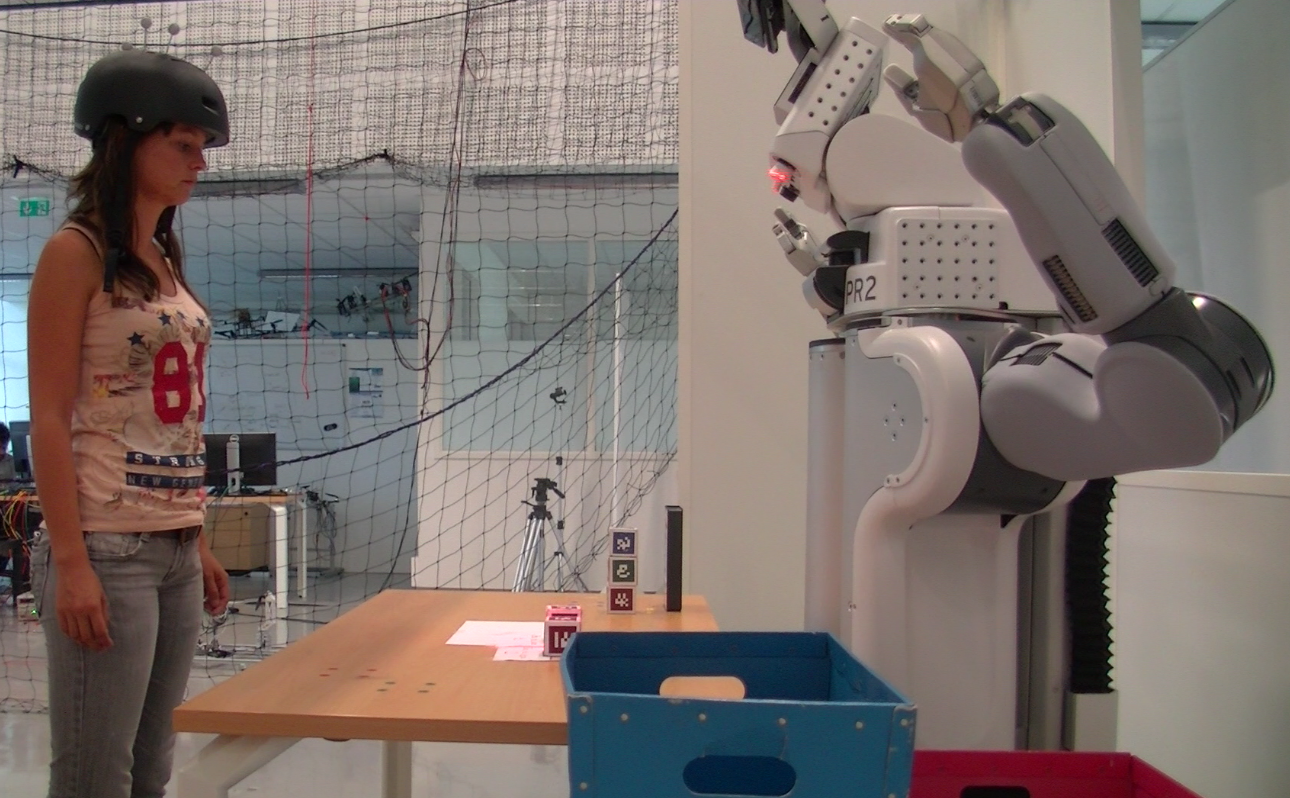
\includegraphics[width=0.7\textwidth]{figs/Chapter5/Scan.png}
    \caption{The PR2 robot interacting with a subject to achieve the task. The robot is scanning the cube before storing it.}
    \label{fig:scan}
\end{figure}


\paragraph{Distraction task:}
We noticed that some subjects tried not to miss any action of the robot (they stayed in front of the robot each time there was a cube to scan and they hurried in the places where they cannot see the robot). Consequently, there was no missing knowledge during the task for these subjects. To ensure that all subjects miss some actions of the robot, at one predefined point of the task, the experimenter asked the subject to leave the task for a while to perform another task. In this task, the subject has to build a construction shown in a picture with Lego bricks. Once the construction achieved, the subject is free to go back to the main task.

\subsection{Protocol}

Each subject of the study had to interact with the robot to achieve the task previously described, and in the four conditions described in Sec.~\ref{sec:task_us}. The order in which they were confronted to the different conditions was randomized. There were four different compositions for the stacks of the human and the robot. The attribution of each composition to a condition was also randomized for each participant.

At their arrival, the participants were introduced to the robot and the environment of the study by the experimenter. Then, participants were asked to read instructions explaining the task and its constraints. The experimenter checked the good understanding of the instructions and showed the emplacements of the different objects of the task. The participants were then asked to perform a quick familiarization task. In this task, the human and the robot had only one cube in their stacks (a blue for the human and a green for the robot). They had to put them in the scan areas, scan them and then store them in the appropriate boxes. There was no tape in the familiarization task. 

After each interaction with the robot (for each condition), the participants were asked to fill a questionnaire in order to evaluate their feeling concerning the robot and the interaction. To do so, several questionnaires have already been developed to evaluate human-robot interaction. \cite{hoffman2013evaluating} allows to evaluate several aspects of the interaction as the "trust" in the robot or the "fluency" of the interaction. It has been used in several studies as \cite{gombolay2015decision} or \cite{dragan2015effects}. However, this questionnaire lacks some aspects needed in our evaluation as "acceptability" or "usability". The Godspeed questionnaire \cite{bartneck2009measurement} allows to measure the perception of the robot by the human with questions relative to "anthropomorphism" or "perceived intelligence". However, this questionnaire is focused on the evaluation of the perception of the robot and lacks parts on the evaluation of the interaction and on the usability of the system. The SUS (System Usability Scale) questionnaire \cite{brooke1986system} allows to measure the interaction of a user with an electronic system with 10 affirmations which subjects need to evaluate with a Lickert scale from "totally agree" to "totally disagree". On the contrary of the Godspeed, the SUS questionnaire measures the usability of the system but lacks of measure concerning the perception of the robot or the interaction. Finally, \cite{heerink2009measuring} presents a toolkit to measure acceptance for assistive social robots. This toolkit is based on the UTAUT (Unified Theory of Acceptance and Use of Technology) questionnaire \cite{venkatesh2003user}. It has been well conceived in order to evaluate the perception and usability of the robot and more particularly for social robots. However, the questionnaire is more oriented toward the perception of the robot than the interaction and the collaboration. 

For this study, like in \cite{heerink2010relating, fischer2016between}, we use a questionnaire that we conceived for the experiment. This questionnaire is composed of several parts:
\begin{itemize}
\item \textit{Verbal:} this part, composed of 3 questions allows to evaluate how the human perceived the verbal interaction with the robot.
\item \textit{Acting:} this part, composed of 3 questions allows to evaluate how the human perceived the decisions of the robot concerning its actions.
\item \textit{Collaboration:} this part, based on \cite{weistroffer2014etude} and composed of 5 questions, allows to evaluate how the human perceived the collaboration between the human and the robot.
\item \textit{Interaction:} this part, based on the AttrakDiff questionnaire \cite{lallemand2015creation} and composed of 5 questions, allows to evaluate how the human perceived the interaction between the human and the robot.
\item \textit{Robot perception:} this part, based on the Godspeed questionnaire \cite{bartneck2009measurement} and composed of 8 questions, allows to evaluate how the human perceived the robot in general.
\end{itemize}
For all the questions, the subject was asked to place himself in a scale of 100 between two antonym adjectives. The English translation of the questionnaire can be found in Appendix~\ref{chap:annexe3}.

In addition to these two questionnaires, after each interaction with the robot (including the familiarization task), we asked participants to answer a small yes/no questionnaire. This questionnaire contains general questions about what happened during the interaction (e.g. "Do you think all the cubes have been scanned?"). The aim of this questionnaire was to remind the key points of the interaction to the subjects (because we noticed during the pre-tests that subjects were kind of "lost" and did not know on what to focus their attention). This questionnaire can also be found in Appendix~\ref{chap:annexe3}.

\subsection{Results}

21 subjects took part in the study. They were all fluent in french and had no significant experience in robotics. The results for the questionnaire evaluating the subjects feeling concerning the robot and the interaction can be found in Fig.~\ref{fig:resUS}. We will discuss the results here bellow.

\begin{figure*}[!h]
\centering
	\subfigure[Scores for the "Verbal" part of the questionnaire]{
        \centering
        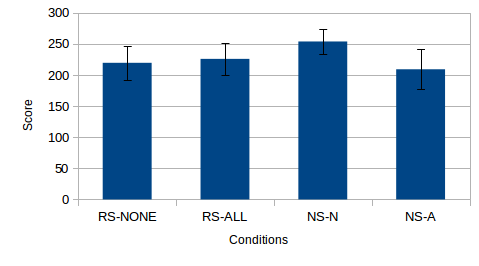
\includegraphics[width=0.45\textwidth]{figs/Chapter5/Verbal.png}
       \label{subfig:resVerbal}
   }
    %~
	\subfigure[Scores for the "Acting" part of the questionnaire]{
        \centering
        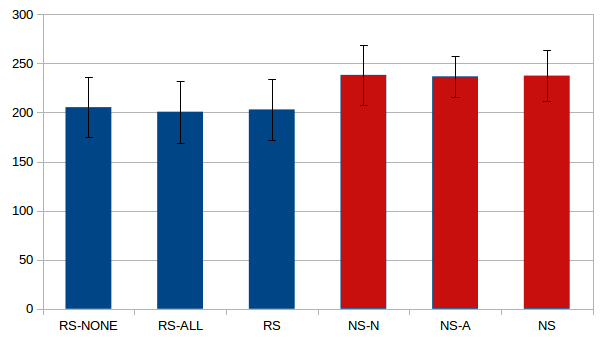
\includegraphics[width=0.45\textwidth]{figs/Chapter5/Acting.png}
       \label{subfig:resActing}
   }
    %~
	\subfigure[Scores for the "Collaboration" part of the questionnaire]{
        \centering
        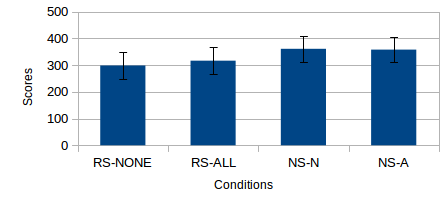
\includegraphics[width=0.45\textwidth]{figs/Chapter5/Collaboration.png}
       \label{subfig:resCollaboration}
   }
    %~
	\subfigure[Scores for the "Interaction" part of the questionnaire]{
        \centering
        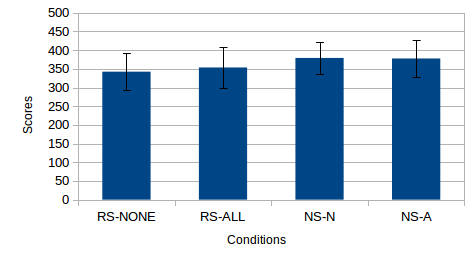
\includegraphics[width=0.45\textwidth]{figs/Chapter5/Interaction.png}
       \label{subfig:resInteraction}
   }
    %~
	\subfigure[Scores for the "Robot perception" part of the questionnaire]{
        \centering
        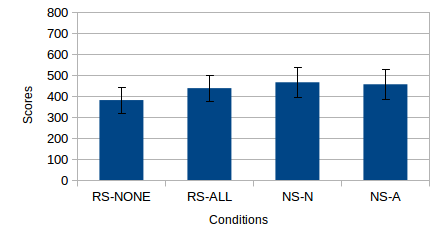
\includegraphics[width=0.45\textwidth]{figs/Chapter5/Robot.png}
       \label{subfig:resRobot}
   }
    \caption{Results on the questionnaire evaluating the subjects feeling concerning the robot and the interaction given to the participants during the user study. The different modes are for the reference system RS-all when the robot verbalizes everything and RS-none when the robot verbalize nothing and for the proposed system NS-N for the negotiation mode and NS-A for the adaptation mode.}
    \label{fig:resUS}
\end{figure*}

\paragraph{Verbal part:} 
The scores of the different modes for the verbal part of the questionnaire can be found in Fig.~\ref{subfig:resVerbal}. The negotiation mode of the new system (NS-N) has been found significantly better than the RS-none condition and the adaptation mode (NS-A) (p < 0.05\footnote{The p values have been calculated with the Student's t-test when the data were normally distributed and with the Wilcoxon test otherwise}). Even if the negotiation mode had a higher score than the RS-all condition, the difference was not found significant. Indeed, when discussing with subjects after the experiment, we found that, for some of them, the fact that the robot was speaking a lot was reassuring. However, they also point out the fact that, even if they found it reassuring the first time, if they had to interact with the robot several time in this mode, they would quickly find it "annoying". Indeed, if we look at some details of the questions asked into the verbal part of the questionnaire, the verbal interaction of the robot have been found more superfluous in the RS-all mode than in the other modes (see Fig.~\ref{subfig:resSuperflus}). Moreover, the verbal interactions in the RS-none mode and the adaptation mode have been found less sufficient than in the other modes (see Fig.~\ref{subfig:resSuficient}). Indeed, the fact that the robot does not inform about its choices (and more particularly concerning the red objects) was found disturbing by the participants. 

\begin{figure*}[!h]
\centering
	\subfigure[Score for the question concerning the verbal interactions where subjects were asked to choose between "insufficient" (0) and "sufficient" (100)]{
        \centering
        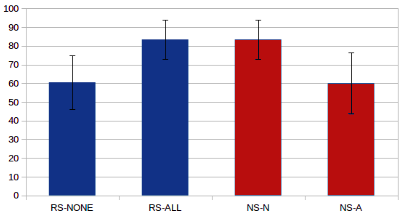
\includegraphics[width=0.45\textwidth]{figs/Chapter5/Suficient.png}
       \label{subfig:resSuficient}
   }
    %~
	\subfigure[Score for the question concerning the verbal interactions where subjects were asked to choose between "superfluous" (0) and "pertinent" (100)]{
        \centering
        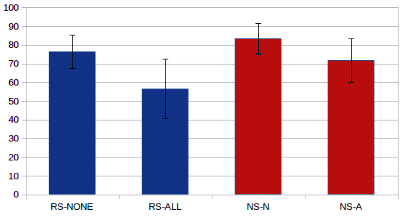
\includegraphics[width=0.45\textwidth]{figs/Chapter5/Superflus.png}
       \label{subfig:resSuperflus}
   }
    \caption{Details of the results on the part of the questionnaire concerning the verbal interactions. The different modes are for the reference system RS-all when the robot verbalizes everything and RS-none when the robot verbalize nothing and for the proposed system NS-N for the negotiation mode and NS-A for the adaptation mode.}
    \label{fig:resUS}
\end{figure*}


\paragraph{Other parts:}
Concerning the rest of the questionnaire, in all other parts, the new system (combination of the negotiation and adaptation modes) had scored significantly higher (p < 0.05) than the reference system (combination of RS-all and RS-none). The difference was particularly visible for the \textit{Acting} part of the questionnaire (p $\simeq$ 0.003). It shows that the algorithms developed for the robot to be able to take the appropriate decisions at the right time during Shared Plan achievement have been appreciated by the subjects.


\section{Conclusion}

The aim of this chapter was to evaluate the algorithms presented in the last two chapters in order to improve the Shared Plan elaboration and execution by the robot. The new system, with its two possible modes (negotiation and adaptation) has been compared to a reference system corresponding to the state of the art before the ameliorations (with two possible options for verbalization). The evaluation has been done both in simulation and with a real study in the real robot. 

Both evaluations have shown that the new system performs better than the old one. In simulation, the adaptation mode performed a little better than the negotiation mode (a little less verbalizations). However, the naive users during the user study preferred the negotiation mode mainly because it was reassuring to have the robot asking when there was a choice. In conclusion, maybe the negotiation mode should be preferred for first or punctual interactions with the robot, and, when the user becomes more used to the robot, the adaptation mode should be preferred.

\ifdefined\included
\else
\bibliographystyle{StyleThese}
\bibliography{These}
\end{document}
\fi
